\documentclass[10pt,a4paper]{article}

\usepackage[utf8]{inputenc}
\usepackage[T1]{fontenc}	
\usepackage[italian]{babel}
\usepackage{amsmath}
\usepackage{amsfonts}
\usepackage{amssymb}
\usepackage{graphicx}

\usepackage[left=2cm,right=2cm,top=2cm,bottom=2cm]{geometry}
\geometry{a4paper}

\usepackage{booktabs} % for much better looking tables
\usepackage{verbatim}
\usepackage{subfig} % make it possible to include more than one captioned figure/table in a single 

\usepackage{fancyhdr} % This should be set AFTER setting up the page geometry
\pagestyle{fancy} % options: empty , plain , fancy
\renewcommand{\headrulewidth}{0pt} % customise the layout...
\lhead{}\chead{}\rhead{}
\lfoot{}\cfoot{\thepage}\rfoot{}

%%% SECTION TITLE APPEARANCE
\usepackage{sectsty}
%\allsectionsfont{\sffamily\mdseries\upshape} % (See the fntguide.pdf for font help)
% (This matches ConTeXt defaults)
% pacchetti che mi fanno schifo ma uso lo stesso (Bob è scemo...)
\usepackage[cdot, thickqspace]{SIunits}
% macro che mi piacciono
\def\code#1{\texttt{#1}}


\title{Esercitazione 4: Amplificatore a transistor}

\author{Gruppo BE \\ Alessandro Candido, Roberto Ribatti}
\date{\today}
\begin{document}
\maketitle

\section{Scopo e strumentazione}
Lo scopo dell'esperienza è realizzare e caratterizzare un amplificatore a transistor, usando un transistor NPN 2N1711.

La strumentazione usata è quella presente sul banco di lavoro, più il suddetto transistor.

\section{Montaggio del circuito e punto di lavoro}
Il circuito è stato realizzato usando i componenti riportati in Tabella~\ref{tab:componenti}

\begin{table}[h!]
\centering
\begin{tabular}{cccc}
$R_1 = \unit{177.1 \pm 1.5}{\kilo\ohm}$ & $R_2 = \unit{18.06 \pm 0.15}{\kilo\ohm}$ & $R_C = \unit{9.93 \pm 0.09}{\kilo\ohm}$ & $R_E = \unit{986 \pm 9}{\ohm}$ \\
$C_{IN} = \unit{230 \pm 10}{\nano\farad}$ & $C_{OUT} = \unit{98 \pm 6}{\nano\farad}$ & $C_E = \unit{100 \pm 10}{\micro\farad}$\\
\end{tabular}
\caption{Valori dei componenti utilizzati per la realizzazione dell'amplificatore}
\label{tab:componenti}
\end{table}

Ad eccezione dell'ultima parte dell'esperienza non è stata usata la resistenza $R_{es}$.

\subsection{Misure e valori attesi}

\paragraph{Punto di lavoro}
Si sono misurate corrente e tensione di quiescenza per determinare il punto di lavoro. Si riporta anche la tensione $V_{CC}$ erogata dall'alimentatore.
\begin{table}[h!]
\centering
\begin{tabular}{ccc}
$V_{CE}^Q = \unit{8.21 \pm 0.05}{\volt}$ & $I_C^Q = \unit{1.058 \pm 0.009}{\milli\ampere}$ & $V_{CC} = \unit{19.85 \pm 0.11}{\volt}$
\end{tabular}
\end{table}

Mentre i valori attesi sono\footnote{exp ad apice sta ad indicare che sono i valori attesi}:

\begin{table}[h!]
\centering
\begin{tabular}{cc}
$V_{CE}^{exp} = \unit{8.03 \pm 0.23}{\volt}$ & $I_C^{exp} = \unit{1.082 \pm 0.022}{\milli\ampere}$
\end{tabular}
\end{table}

Per calcolarli si è usato che $V_{BE} = \unit{625 \pm 4}{\milli\volt}$, cioè quanto abbiamo misurato.

\paragraph{Tensioni ai terminali del transistor}
Le tensioni misurate sui terminali del transistor sono le seguenti.

\begin{table}[h!]
\centering
\begin{tabular}{cccc}
$V_B = \unit{1.692 \pm 0.009}{\volt}$ & $V_E = \unit{1.070 \pm 0.006}{\volt}$ & $V_{BE} = \unit{625 \pm 4}{\milli\volt}$ & $V_{C} = \unit{9.28 \pm 0.06}{\volt}$
\end{tabular}
\end{table}

Mentre per i valori attesi si è ottenuto:

\begin{table}[h!]
\centering
\begin{tabular}{ccc}
$V_B^{exp} = \unit{1.701 \pm 0.019}{\volt}$ & $V_E^{exp} = \unit{1.076 \pm 0.20}{\volt}$ & $V_{C}^{exp} = \unit{9.10 \pm 0.22}{\volt}$
\end{tabular}
\end{table}

Non si riporta il valore atteso di $V_{BE}$ in quanto è stato usato proprio il valore misurato per ricavare gli altri. Si nota però che approssimativamente corrisponde ai valori tipici noti di $\sim \unit{0.6-0.7}{\volt}$
% non so se ha veramente senso includere quest'ultima parte
% pensiamo abbia senso, stiamo a vedere come la valutano

\paragraph{Compatibilità} Le misure sono tutte compatibili con i valori attesi, ad eccezione della corrente di collettore che risulta poco inferiore alla previsione (la differenza fra $I_C$ misurata e attesa è $\unit{-24 \pm 23}{\micro\ampere}$).

\paragraph{Formule} Si riportano le formule usate per calcolare le tensioni e le correnti attese, noti i valori delle resistenze e $V_{BE}$ e $V_{CC}$, oltre ovviamente al guadagno in corrente $h_{FE}$; in particolare si riportano quelle per $V_B$ e $I_B$, le altre seguono direttamente da queste, senza ulteriori conti.
\begin{align*}
I_B &= \frac{\frac{R_2}{R_1 + R_2} V_{CC} - V_{BE}}{R_E (h_{FE} + 1) + R_1 // R_2} \\
V_B &= V_{BE} + R_E (h_{FE} + 1) I_B
\end{align*}

\subsection{Partitore $R_1-R_2$}
Il valore di $I_B$ è dunque $I_C/h_{FE} = \unit{8.13 \pm 0.15}{\micro\ampere}$, mentre la corrente che passa per la resistenza $R_1$ è pari a $I_1 = \unit{102.5 \pm 1.1}{\micro\ampere}$, per cui $I_B$ è $\sim 8\%$ della corrente che scorre nel partitore. In questo caso non si può affermare che il partitore sia stiff, infatti $I_B$ è solo un ordine di grandezza più piccola della corrente $I_1$, per cui il rapporto di partizione non è indipendente dalla richiesta di corrente del transistor.

\section{Risposta a segnali sinusoidali a frequenza fissa}
Si è misurato il guadagno per varie ampiezze del circuito amplificatore riportato sulla scheda, escludendo $C_E$ ed $R_E$ (cioè disconnettendoli).

\paragraph{Inversione di fase} Si è osservato che il segnale in uscita risultava in opposizione di fase rispetto al segnale in ingresso, come atteso. Si riporta in \figurename{\ref{fig:sfasamento}} la relativa schermata dell'oscilloscopio.

\begin{figure}[h!]
	\centering
	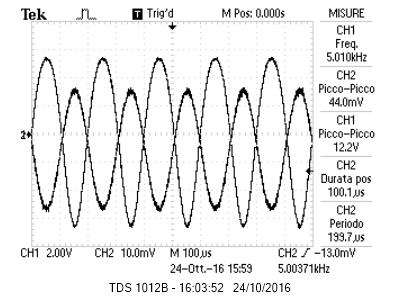
\includegraphics[width=0.54\textwidth]{../oscilloscopio/sfasamento.jpg}
	\caption{Sfasamento del segnale in uscita rispetto a quello in ingresso}
	\label{fig:sfasamento}
\end{figure}

\paragraph{Guadagno e linearità del circuito}
Si è fittato il guadagno in tensione del circuito $A_V$ ottenendo per esso un valore di $9.62 \pm 0.09$, con un $\chi^2 / ndof = 10.1 / 26$. Si può affermare, dal grafico degli scarti, che la linearità è preservata per le tensioni d'ingresso che non portano il transistor in clipping.

\begin{figure}
\centering
\begin{minipage}[c]{0.7\textwidth}
\centering
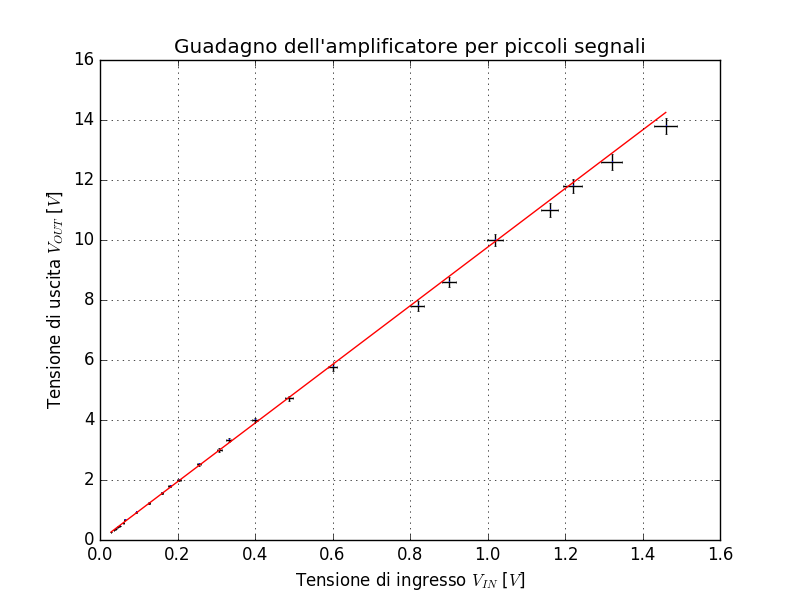
\includegraphics[width=\textwidth]{../grafici/fit_guadagnopiccolisegnali.pdf}
\end{minipage}
\caption{Grafico e scarti del fit del guadagno del circuito per piccoli segnali}
\end{figure}

\paragraph{Clipping}
Il segnale in uscita risultava simmetrico fino ad ampiezze di $\sim \unit{1.7}{\volt}$ in ingresso.
% forse avremmo potuto stimare un errore su quei 1.7 V, magari possiamo stimarlo "a memoria"
% nessuno ci ha chiesto una misura quantitativa, era richiesto solo un resoconto qualitativo, quindi lasciamo il circa anziché l'errore, però stiamo a vedere come ce la valutano
Per intensità maggiori si osservava che l'uscita era tagliata dal basso. Questo taglio del segnale (riportato in \figurename{\ref{fig:clipping}}) corrisponde ad un regime di funzionamento del transistor diverso da quello attivo, in cui sarebbe preservata la linearità.

Si può identificare tale regime con quello di saturazione. Infatti quando scorre una maggiore corrente nel collettore si ha una caduta di potenziale maggiore su $R_C$, e dunque una minore tensione in uscita. Arrivando in saturazione il transistor non è in grado di erogare una corrente maggiore, e quindi la caduta di potenziale si assesta su un certo valore, finché la richiesta di corrente non diminuisce e il segnale in uscita riprende a salire.

\begin{figure}[h!]
	\centering
	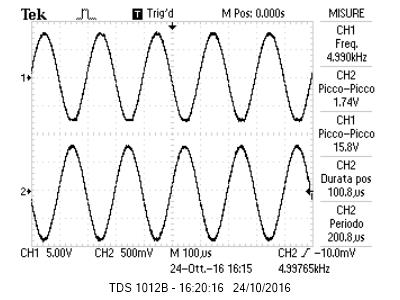
\includegraphics[width=0.54\textwidth]{../oscilloscopio/firstclipbasso.jpg}
	\caption{}
	\label{fig:clipping}
\end{figure}

Si era trovato che il punto di lavoro del transistor era fissato ad una corrente di collettore relativamente bassa, e quindi vicina al regime di interdizione. Tracciando la retta di carico si nota però che la pendenza di questa è relativamente piccola in valore assoluto, per cui, per ottenere spostamenti verticali\footnote{sul grafico delle curve caratteristiche di collettore, quindi piccole variazioni di $I_C$} anche ridotti, che porterebbero il transistor a lavorare in interdizione, si hanno notevoli spostamenti orizzontali\footnote{cioè variazioni di $V_{CE}$}, che portano dunque il transistor a lavorare in saturazione per segnali in ingresso di ampiezza minore rispetto a quelli che sarebbero necessari a portarlo in interdizione.
% poi ci metto qualche numerello per rendere la cosa più quantitativa
% come per il commento precedente non era richiesto nulla se non qualitativo, stiamo a vedere

Per segnali in ingresso di ampiezza ancora maggiore ottengo il taglio dell'uscita anche dall'alto, arrivando a oscillare quindi tra i due regimi di saturazione e interdizione, si veda \figurename{\ref{fig:clippingdoppio}}

\begin{figure}[h!]
	\centering
	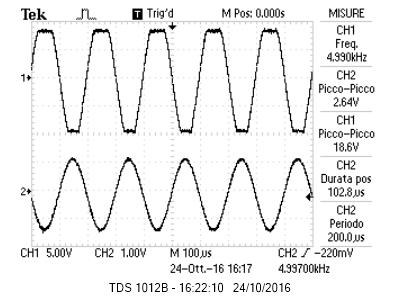
\includegraphics[width=0.54\textwidth]{../oscilloscopio/clipall.jpg}
	\caption{}
	\label{fig:clippingdoppio}
\end{figure}

\subsection{Impedenza d'ingresso}
I valori ottenuti di $V_1$ e $V_2$, con riferimento alla scheda, sono rispettivamente $\unit{1.360 \pm 0.008}{\volt}$ e $\unit{700 \pm 4}{\milli\volt}$, e per misurarle si è usata una resistenza $R_S = \unit{14.70 \pm 0.13}{\kilo\ohm}$.
Si è così ottenuta un'impedenza d'ingresso pari a $R_{in} = \unit{15.6 \pm 0.3}{\kilo\ohm}$.

\subsection{Impedenza d'uscita}
Come nel paragrafo precedente: $V_1 = \unit{12.8 \pm 0.07}{\volt}$, $V_2 = \unit{6.56 \pm 0.04}{\volt}$, $R_L = \unit{9.87 \pm 0.09}{\kilo\ohm}$.
Si è così ottenuta un'impedenza d'uscita pari a $R_{out} = \unit{9.39 \pm 0.19}{\kilo\ohm}$.

\section{Risposta in frequenza}

Si è misurata la risposta in frequenza del circuito in esame in un range tra $\unit{10}{\hertz}$ ed $\unit{1}{\mega\hertz}$ con una tensione di ingresso costante di $\unit{1.00 \pm 0.03}{\volt}$. Di seguito si riportano i dati raccolti e il diagramma di Bode da questi ricavato. In tutte le tabelle e nell'analisi dati sono state ignorate le incertezze di calibrazione, e sono stati considerati solo gli errori di lettura.

\begin{figure}[h!]
	\centering
	\begin{minipage}[c]{0.3\textwidth}
		\centering
		\resizebox{\textwidth}{!}{
			\input{../tabelle/tab_f_domain.txt}}
		\captionof{table}{Dati raccolti}
	\end{minipage}
	\begin{minipage}[c]{0.69\textwidth}
		\centering
		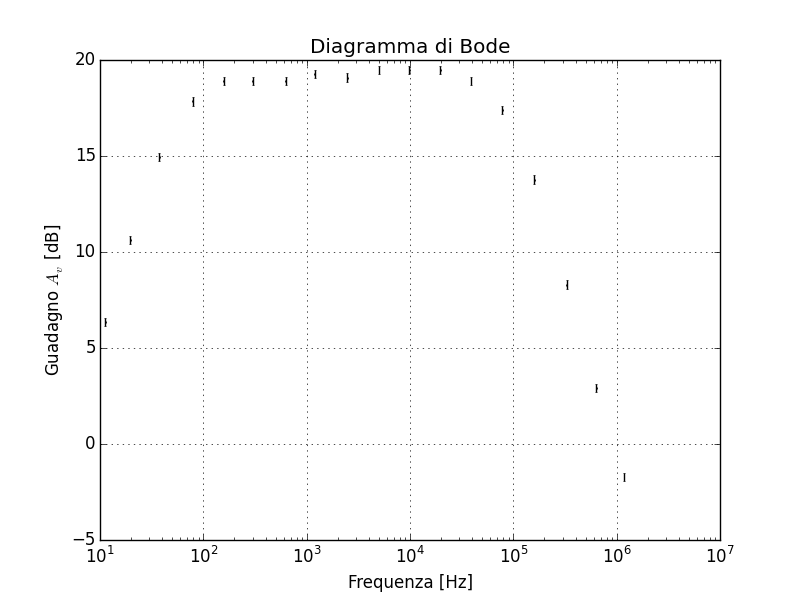
\includegraphics[width=1.1\textwidth]{../grafici/fast_plot_f_domain.pdf}
		\caption{Risposta in frequenza}
		\label{early}
	\end{minipage}
\end{figure}

Il grafico mostra un comportamento divisibile in tre bande di risposta:
\begin{itemize}
	\item {basse frequenze ($\lesssim$ \unit{100}{\hertz})} Il diagramma di Bode mostra un comportamento lineare, a queste frequenze le impedenze dei condensatori $C_{OUT}$ e $C_{IN}$ nel circuito non è trascurabile e diminuisce il guadagno del circuito. 
	
	In particolare si comportano entrambi come passa basso, il primo condensatore $C_{IN}$ vede la resistenza di ingresso del circuito $R_{in}$ misurata precedentemente, mentre il secondo condensatore $C_{OUT}$ vede l'impedenza di ingresso dell'oscilloscopio, che è stata misurata nella prima esperienza ($R_{osc} = \unit{1.00 \pm 0.02}{\mega\ohm}$). Le frequenze di taglio attese sono $f_{in}=\unit{44.4 \pm 2.1}{\hertz}$ e $f_{out}=\unit{1.62 \pm 0.10}{\hertz}$, la frequenza di taglio del circuito complessivo può essere in questo caso ($f_{out} << f_{in}$) approssimata a $f_{low} \simeq f_{in} + f_{out} = \unit{46.0 \pm 2.1}{\hertz}$
	
	
	\item {medie frequenze ($\unit{100}{\hertz} \lesssim f \lesssim \unit{100}{\kilo\hertz}$)} In questo range di frequenze il guadagno del circuito è costante, tutte le approssimazioni che si fanno classicamente per la risoluzione del circuito sono valide e il comportamento atteso è $A_v = R_C/R_E = 10.07\pm0.13$.
	
	\item {alte frequenze ($\gtrsim \unit{100}{\kilo\hertz}$)} Anche qui il diagramma di Bode mostra un comportamento lineare, la diminuzione del guadagno è dovuta alla capacità della giunzione (in particolare la giunzione CB il cui valore dal datasheet è $\sim \unit{20}{\pico\farad}$) che per effetto Miller risulta amplificata di un fattore $\sim A_v$. Una stima del valore atteso della frequenza di taglio è $f_{high} \sim \unit{70}{\kilo\hertz}$.
\end{itemize}

Si è stimata la frequenza di taglio del circuito misurando la frequenza per la quale si ha un guadagno di $\unit{-3}{\deci\bel}$ e si è stimato l'errore valutando quando, al variare della frequenza, si misurava una variazione apprezzabile della tensione di uscita.
I risultati ottenuti sono stati: $f_1 = \unit{51 \pm 5}{\hertz}$ e $f_2= \unit{92 \pm 10}{\kilo\hertz}$.
Si è quindi provato a fittare il comportamento a basse e alte frequenze nell'ipotesi fatta precedentemente che il circuito si comporti come se fosse in serie ad un filtro passa alto/basso rispettivamente.
I risultati dei fit sono stati:
\begin{table}[h!]
	\centering
\begin{tabular}{ccc}
$f_{low}=\unit{48.7 \pm 1.1}{\hertz}$ & $A_v = 9.16 \pm 0.08$ & $\chi^2/ndof = 7.3 / 10$ \\
$f_{high}=\unit{100.3 \pm 1.8}{\kilo\hertz}$ & $A_v = 9.19 \pm 0.08$ & $\chi^2/ndof = 19 / 11$
\end{tabular}
\end{table}

Di seguito riportiamo i grafici dei fit eseguiti.
\begin{figure}[h!]
	\centering
	\begin{minipage}[c]{0.49\textwidth}
		\centering
		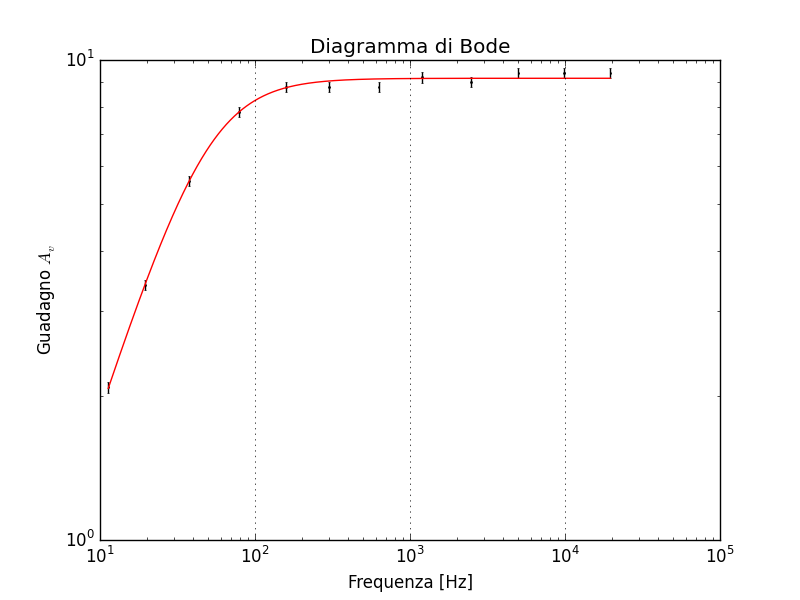
\includegraphics[width=\textwidth]{../grafici/fit_low_frequency.pdf}
		\caption{Fit basse frequenze}
	\end{minipage}
	\begin{minipage}[c]{0.49\textwidth}
		\centering
		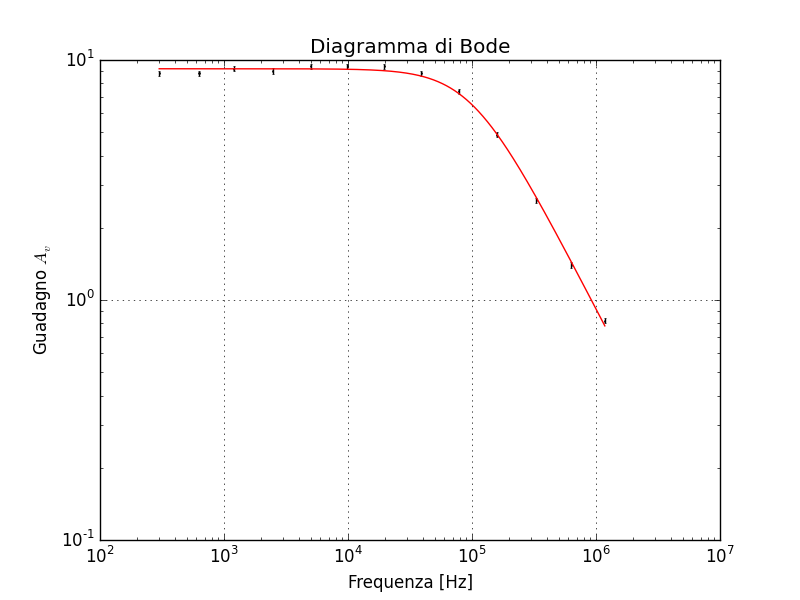
\includegraphics[width=\textwidth]{../grafici/fit_high_frequency.pdf}
		\caption{Fit alte frequenze}
	\end{minipage}
\end{figure}

\paragraph{Conclusioni}
Tutte le misure di $f_{low}$ sono compatibili tra loro e con il valore atteso a meno di $1\sigma$, anche le misure di $f_{high}$ sono compatibili tra loro e concordano almeno in ordine di grandezza con la stima del valore atteso.
\section{Aumento del guadagno}

Si è inserita la resistenza $Res = \unit{100.7 \pm 1.1}{\ohm}$ nel circuito in \figurename{\ref{stocazzo}} e si è proceduto alla misura del guadagno al variare delle tensione di ingresso (a frequenza costante di $\unit{5.03 \pm 0.05}{\kilo\hertz}$). I dati raccolti sono riportati di seguito.

\begin{figure}[h!]
	\centering
	\begin{minipage}[c]{0.3\textwidth}
		\centering
		\resizebox{\textwidth}{!}{
			\input{../tabelle/tab_C_E.txt}}
		\captionof{table}{Dati raccolti}
		\label{data}
	\end{minipage}
	\begin{minipage}[c]{0.69\textwidth}
		\centering
		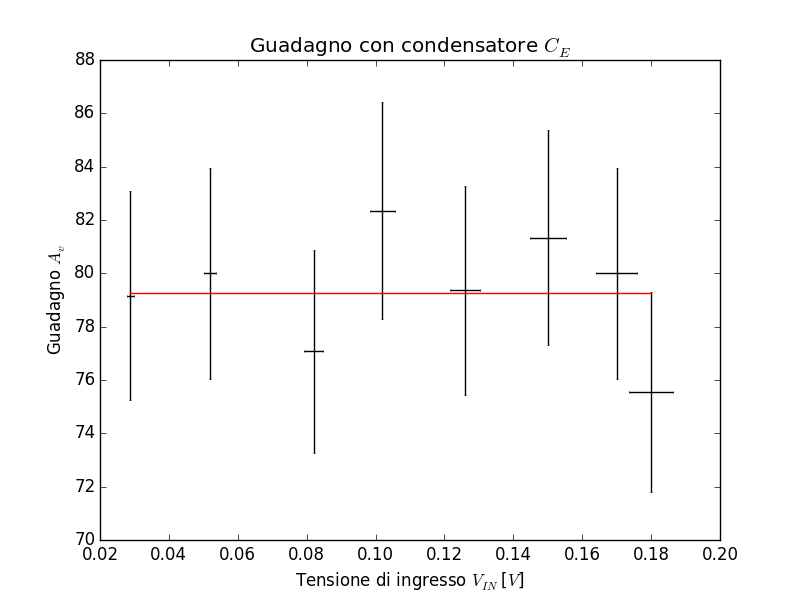
\includegraphics[width=1.1\textwidth]{../grafici/fit_C_E.pdf}
		\caption{Risposta in frequenza}
	\end{minipage}
\end{figure}

In \tablename{\ref{data}} sono riportate le misure e il loro errore di lettura, ignorando l'errore di calibrazione ($\sim 3\%$) poichè 

Il guadagno è stato valutato fittando con una retta $V_{IN}$ in funzione di $V_{OUT}$. I risultati sono stati $A_v = -80.5 \pm 2.6$, un intercetta di $\unit{0.05 \pm 0.16}{\volt}$ e un $\chi^2/ndof = 4.5/6$.  Come è chiaro $A_v$ non è compatibile con il risultato della formula $A_v = -R_C/Res = 98.6 \pm 1.4$ perché questa formula è il risultato dell'approssimazione $h_{fe}*Z_c >> h_{ie}$, che non è valida in questo caso poichè $h_{fe} * Z_c \simeq h_{fe} * Res \simeq \unit{130 * 100}{\ohm} = \unit{13}{\kilo\ohm} $ che è confrontabile a $h_{ie}$ che secondo il datasheet vale $\sim \unit{4}{\kilo\ohm}$, applicando la formula non approssimata $A_v = -h_{fe}*R_C/(h_{fe}*Z_c + h_{ie}) \simeq 77$ che è in ragionevole accordo con il valore trovato.

\section{Appendice: Dati}
Si riportano qui le tabelle di dati usati per i fit e i grafici.


\end{document}
